%TODO: ARREGLAR EJERCICIO 1B
\documentclass{article}
\usepackage[utf8]{inputenc}
\usepackage[spanish]{babel}
\usepackage{graphicx, graphics, float, hyperref}
\usepackage{listings}
\usepackage[a4paper, total={6in, 10in}]{geometry}

\title{SSO Práctica 1 Sesión 3}
\author{Andrés Merlo Trujillo}
\date{}
\hypersetup{
    colorlinks=true,
    linkcolor=black,
}

\begin{document}

\maketitle

\tableofcontents

\newpage
%\addcontentsline{toc}{section}{Ejercicio 1}
%\section*{Ejercicio 1}
%\begin{figure}[H]
%    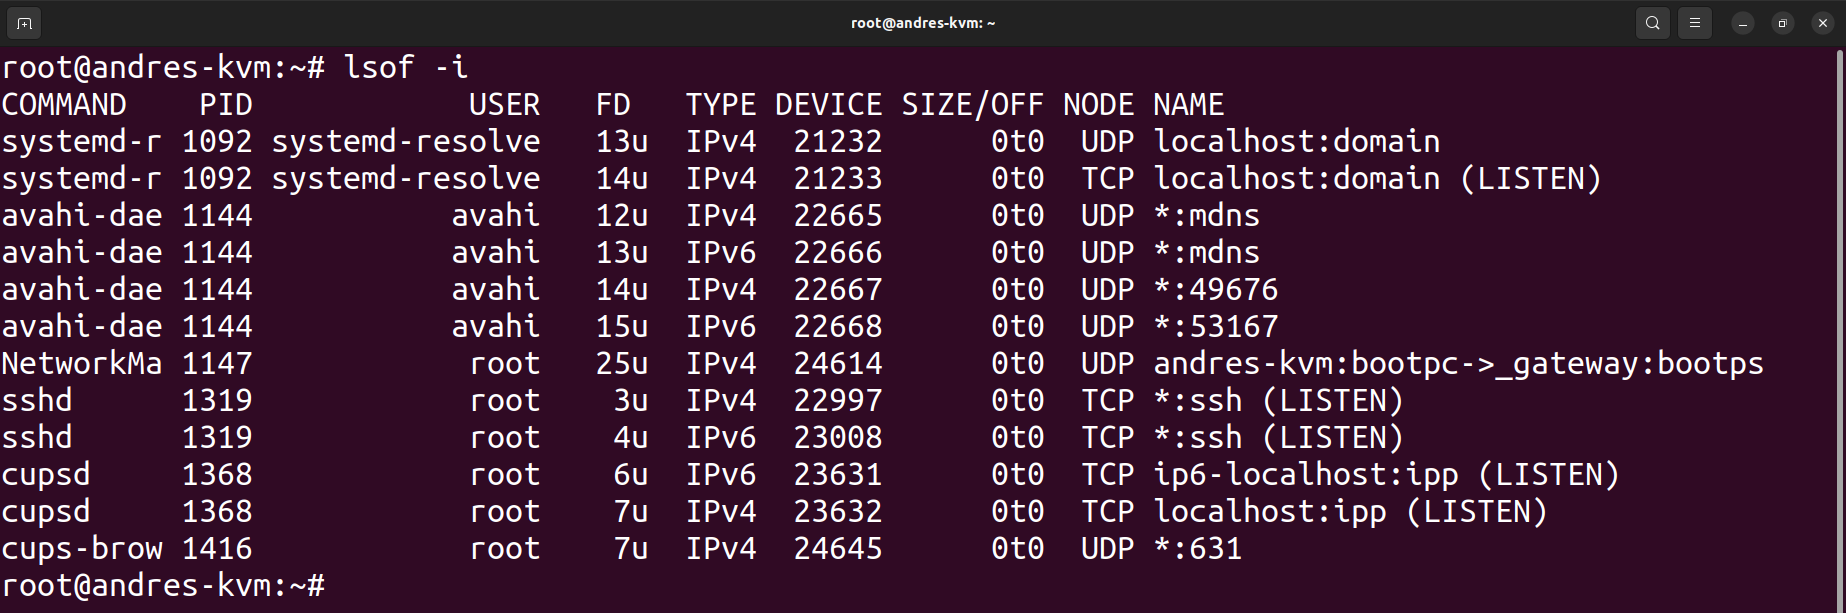
\includegraphics[width=\textwidth]{imagenes/lsofi.png}
%\end{figure}

\addcontentsline{toc}{section}{Ejercicio 1}
\section*{Ejercicio 1}

\addcontentsline{toc}{subsection}{Apartado A}
\subsection*{Apartado A}

Para crear las claves personales es necesario ejecutar la orden \verb|gpg --gen-key|. Ahora pedirá una serie de información que es necesario rellenar como el nombre o el correo.

%foto de nombre y apellidos.
\begin{figure}[H]
    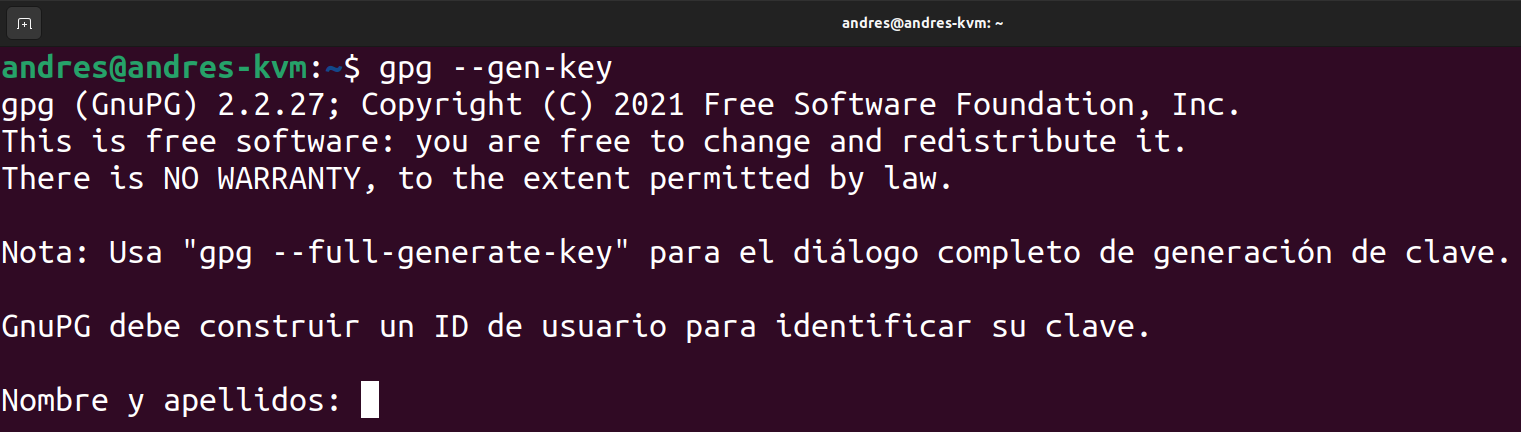
\includegraphics[width=\textwidth]{imagenes/Captura desde 2022-10-19 16-42-45.png}
\end{figure}

A continuación aparece un sumario de los datos rellenados y al aceptarlos aparece un cuador de texto para introducir la contraseña. A continuacion pide al usuario realizar diversas cosas para generar entropia y que la clave sea lo mas aleatoria posible como mover el raton, realizar actividad de red y de disco, etc.

\begin{figure}[H]
    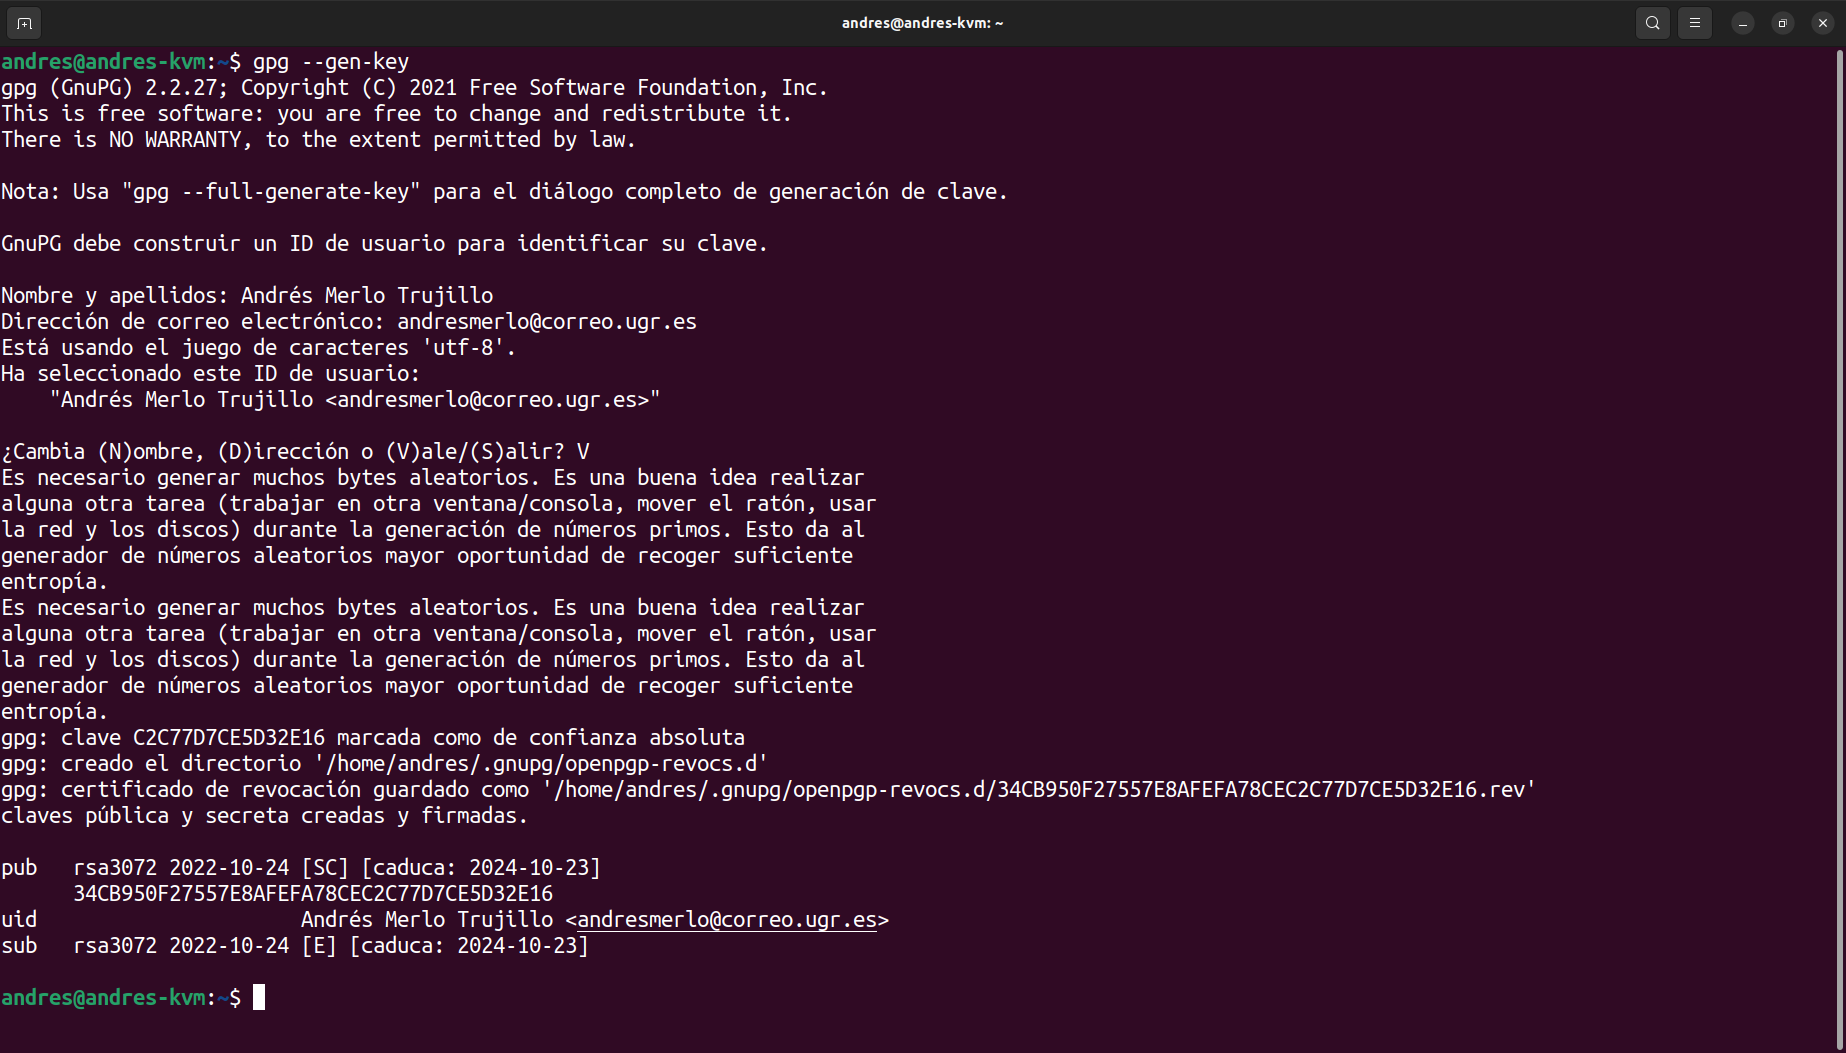
\includegraphics[width=\textwidth]{imagenes/Portatil/Captura desde 2022-10-24 11-46-02.png}
\end{figure}

Y ahora para mostrar las claves publicas se utiliza el comando \verb|gpg --list-keys|:

%Captura desde 2022-10-19 16-55-18
\begin{figure}[H]
    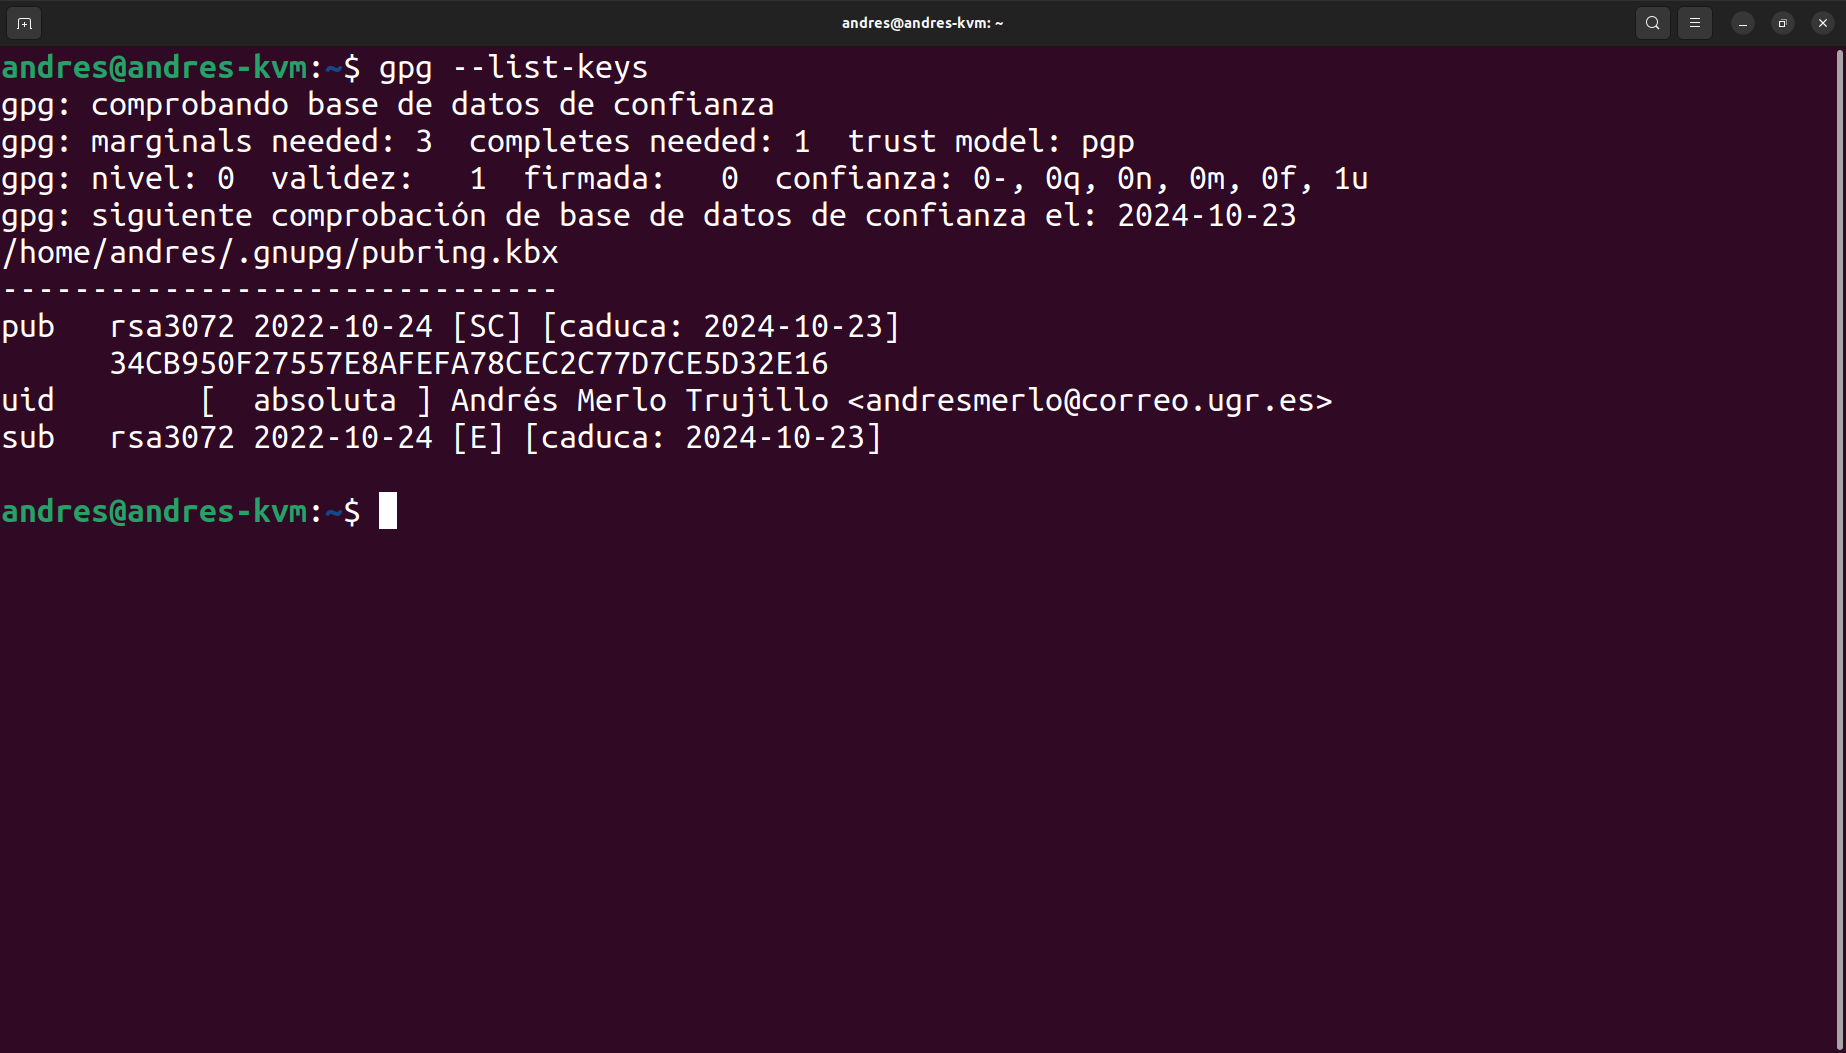
\includegraphics[width=\textwidth]{imagenes/Portatil/Captura desde 2022-10-24 11-46-16.png}
\end{figure}

Y para mostrar las claves privadas se utiliza el comando \verb|gpg --list-secret-keys|:

%Captura desde 2022-10-19 16-55-26
\begin{figure}[H]
    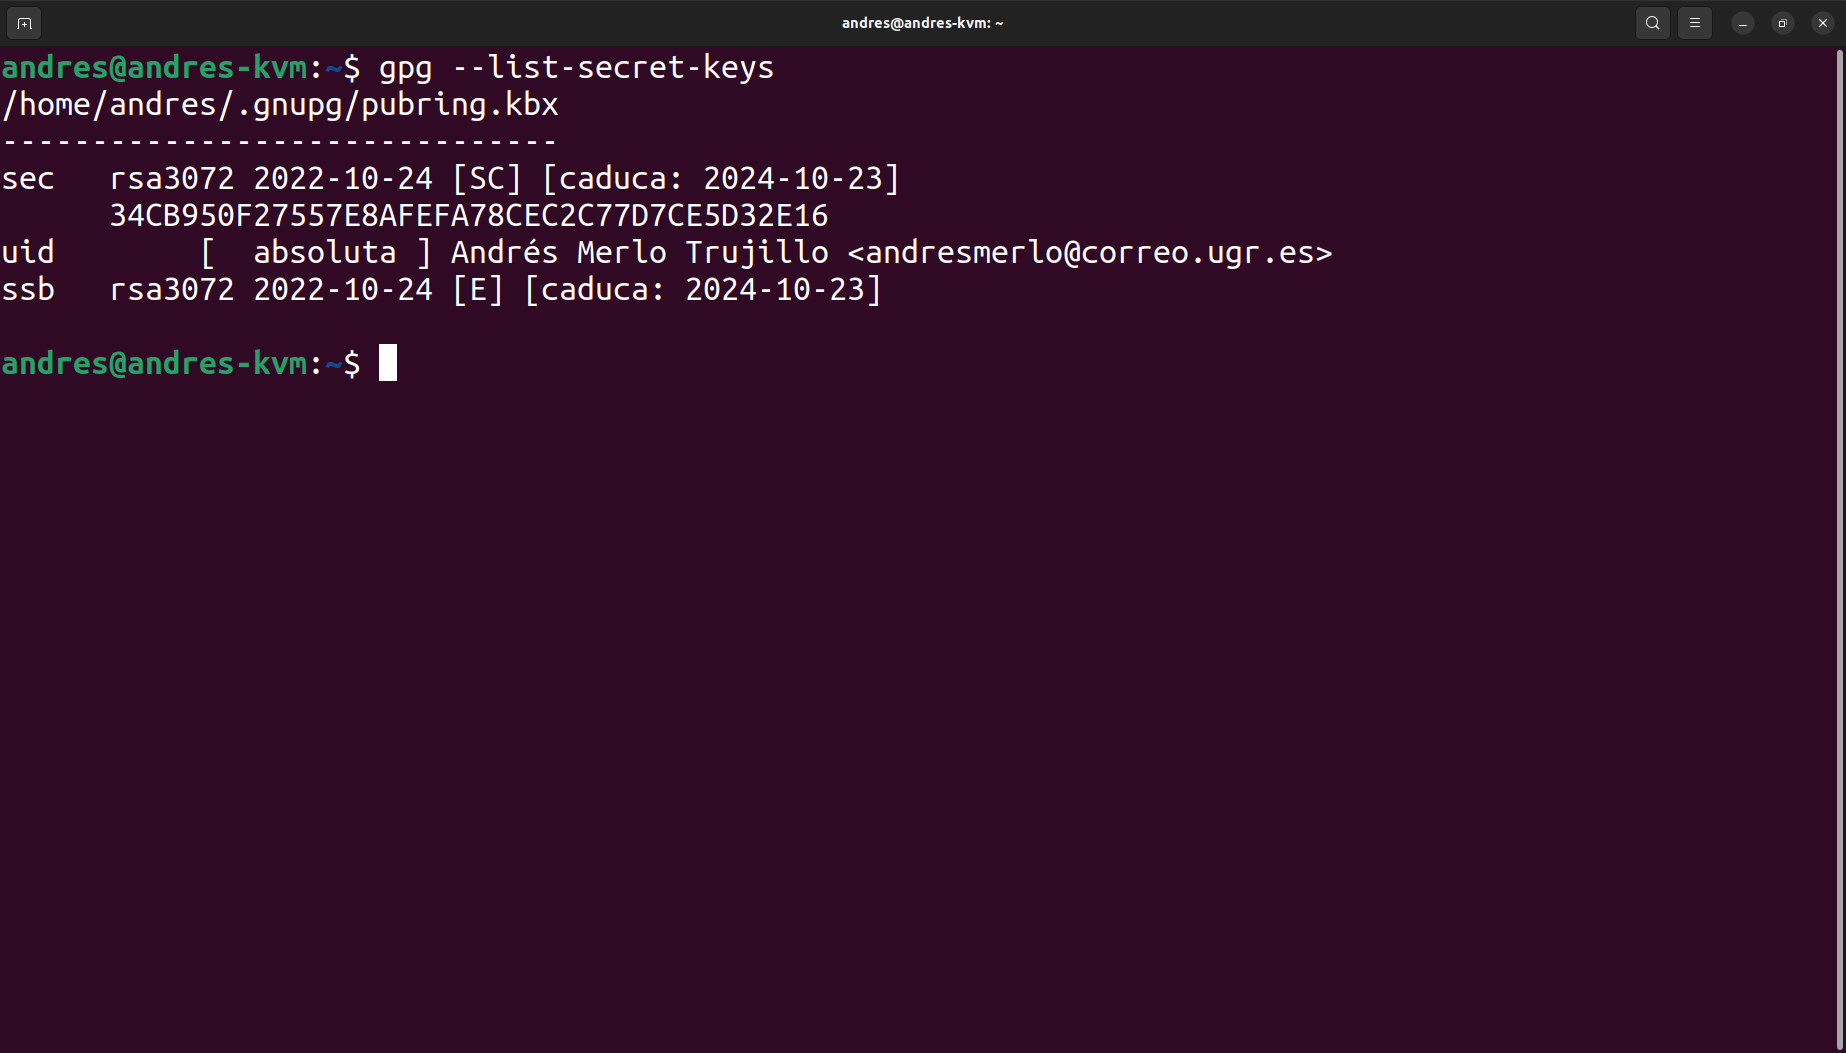
\includegraphics[width=\textwidth]{imagenes/Portatil/Captura desde 2022-10-24 11-46-25.png}
\end{figure}

\addcontentsline{toc}{subsection}{Apartado B}
\subsection*{Apartado B}

Primero voy a crear un archivo de texto cualquiera como el siguiente:

%Captura desde 2022-10-19 16-57-15
\begin{figure}[H]
    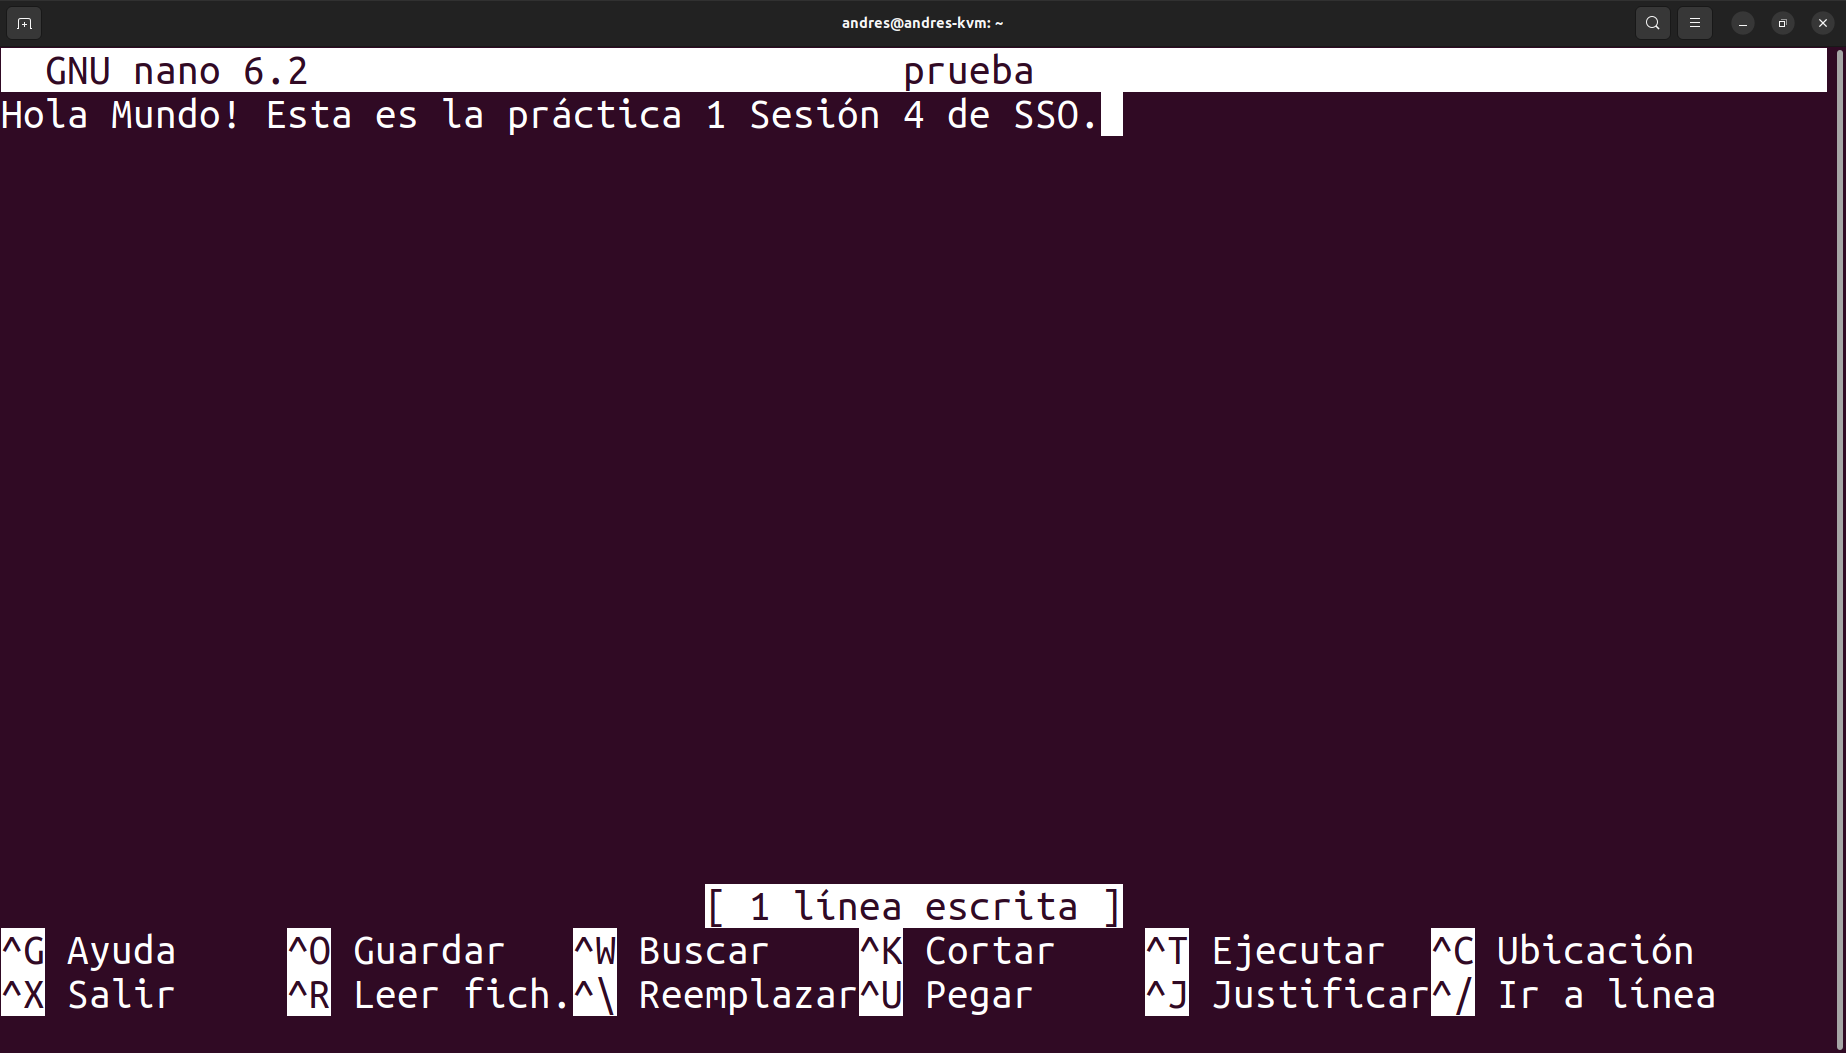
\includegraphics[width=\textwidth]{imagenes/Captura desde 2022-10-19 16-57-15.png}
\end{figure}

Y ahora para cifrar el archivo se utiliza el comando \verb|gpg --armor --recipient correo --encrypt file|. Para ello, en la parte de ``recipient'' es necesairo poner el correo que se haya usado para crear las claves en el ejercicio anterior, o cualquier otro que se encuentre en algún servidor como \verb|keyserver.ubuntu.com| o incluso importado localmente entre personas. Yo voy a realizar la primera de todas, encriptarlo con mi propia clave para mi correo.

Esto generara un fichero con la extension ``.asc'' el cual, si se abre, contiene lo siguiente:

%Captura desde 2022-10-19 17-06-08
\begin{figure}[H]
    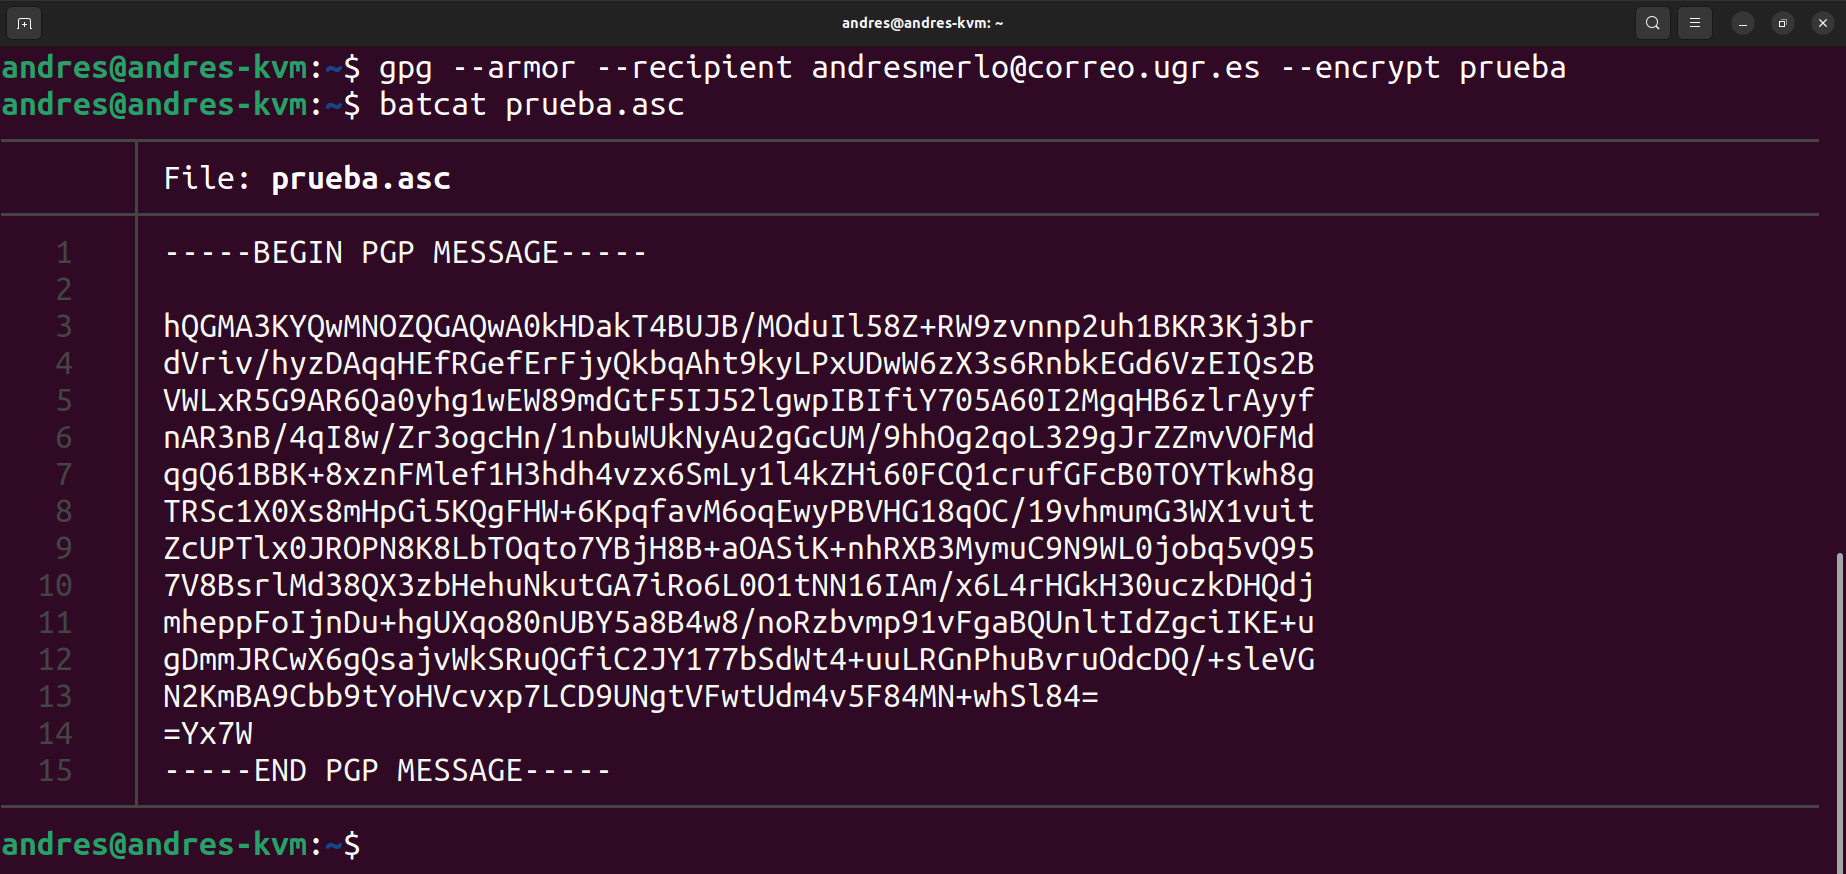
\includegraphics[width=\textwidth]{imagenes/Portatil/Captura desde 2022-10-27 18-34-40.png}
\end{figure}


Por ultimo, para descifrar el mensaje se utiliza la orden \verb|gpg --decrypt prueba.asc|, se pedira la contraseña que se inserto al crear las claves.

%Captura desde 2022-10-19 17-07-30
\begin{figure}[H]
    \centering
    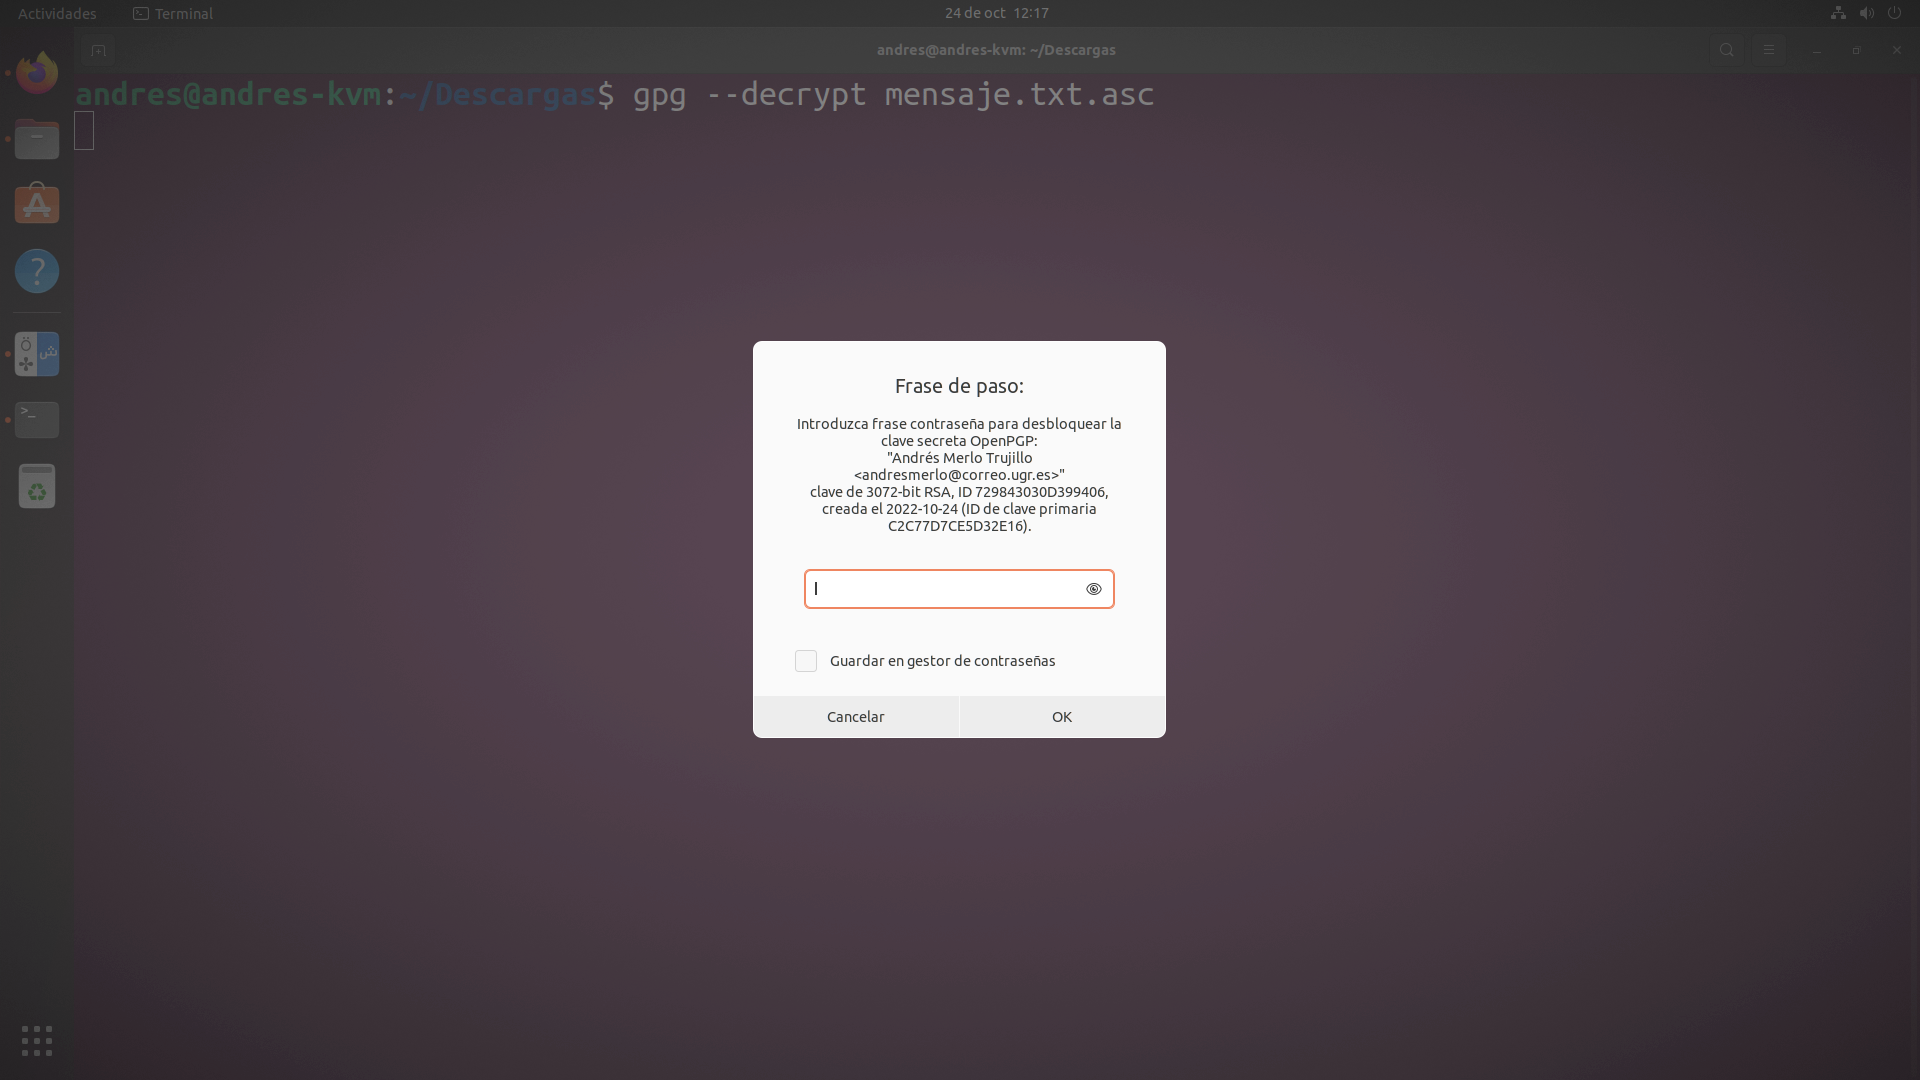
\includegraphics[width=0.6\textwidth]{imagenes/Portatil/Captura desde 2022-10-24 12-17-29.png}
\end{figure}

%Captura desde 2022-10-19 17-07-50
\begin{figure}[H]
    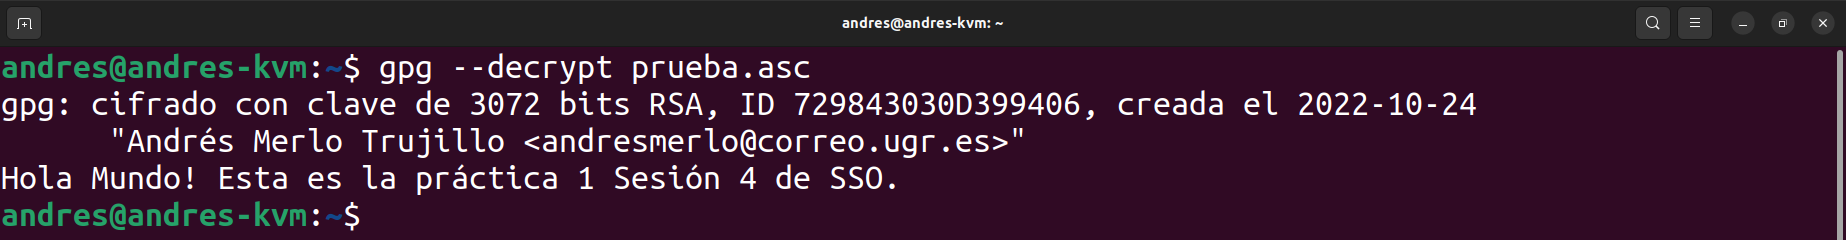
\includegraphics[width=\textwidth]{imagenes/Portatil/Captura desde 2022-10-27 18-35-01.png}
\end{figure}


\addcontentsline{toc}{subsection}{Apartado C}
\subsection*{Apartado C}

Me he juntado con Carlos Salas Eiroa (csalaseiroa@correo.ugr.es) para mandarnos archivos cifrados a cada uno.

Para que él pueda obtener mi clave publica, es necesario subirla a un servidor como \url{https://keyserver.ubuntu.com/}. Para ello, necesito obtener el ID de la clave publica mia en formato corto con la orden \verb|gpg --list-keys --keyid-format SHORT|.


\begin{figure}[H]
    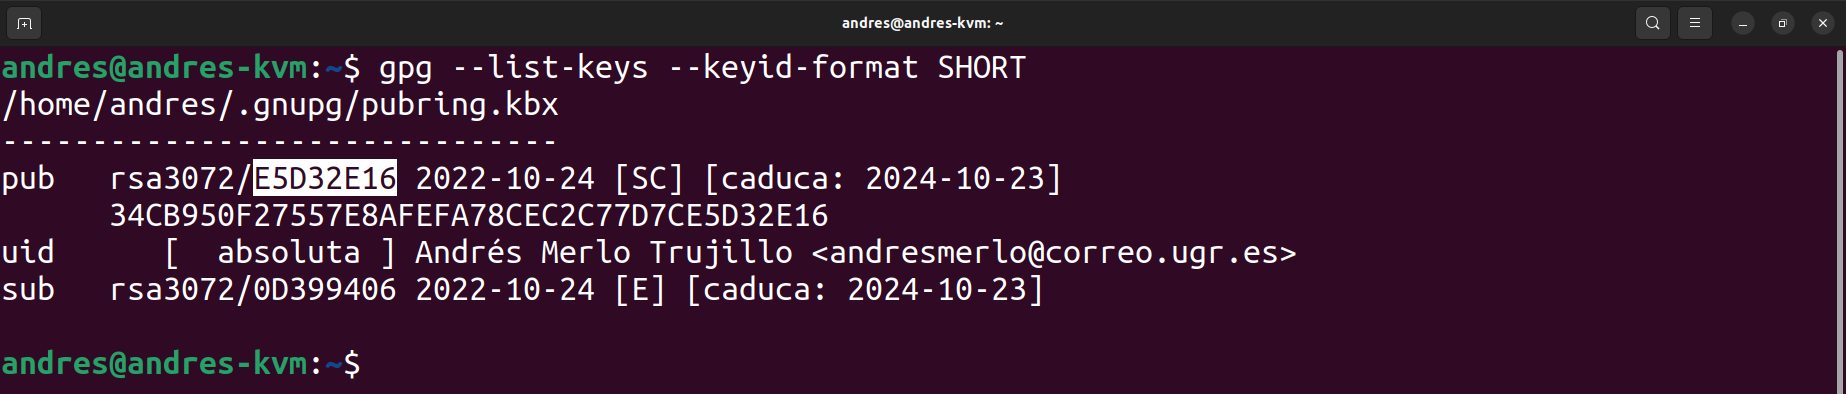
\includegraphics[width=\textwidth]{imagenes/Portatil/Captura desde 2022-10-24 11-54-58.png}
    \caption{El ID corto se encuentra en la tercera linea despues de ``rsa3072/''.}
\end{figure}

Y una vez obtenido el ID en formato corto, con la orden \verb|gpg --send-keys --keyserver keyserver.ubuntu.com SHORT_ID| se envia al servidor.

%Captura desde 2022-10-24 11-58-08
\begin{figure}[H]
    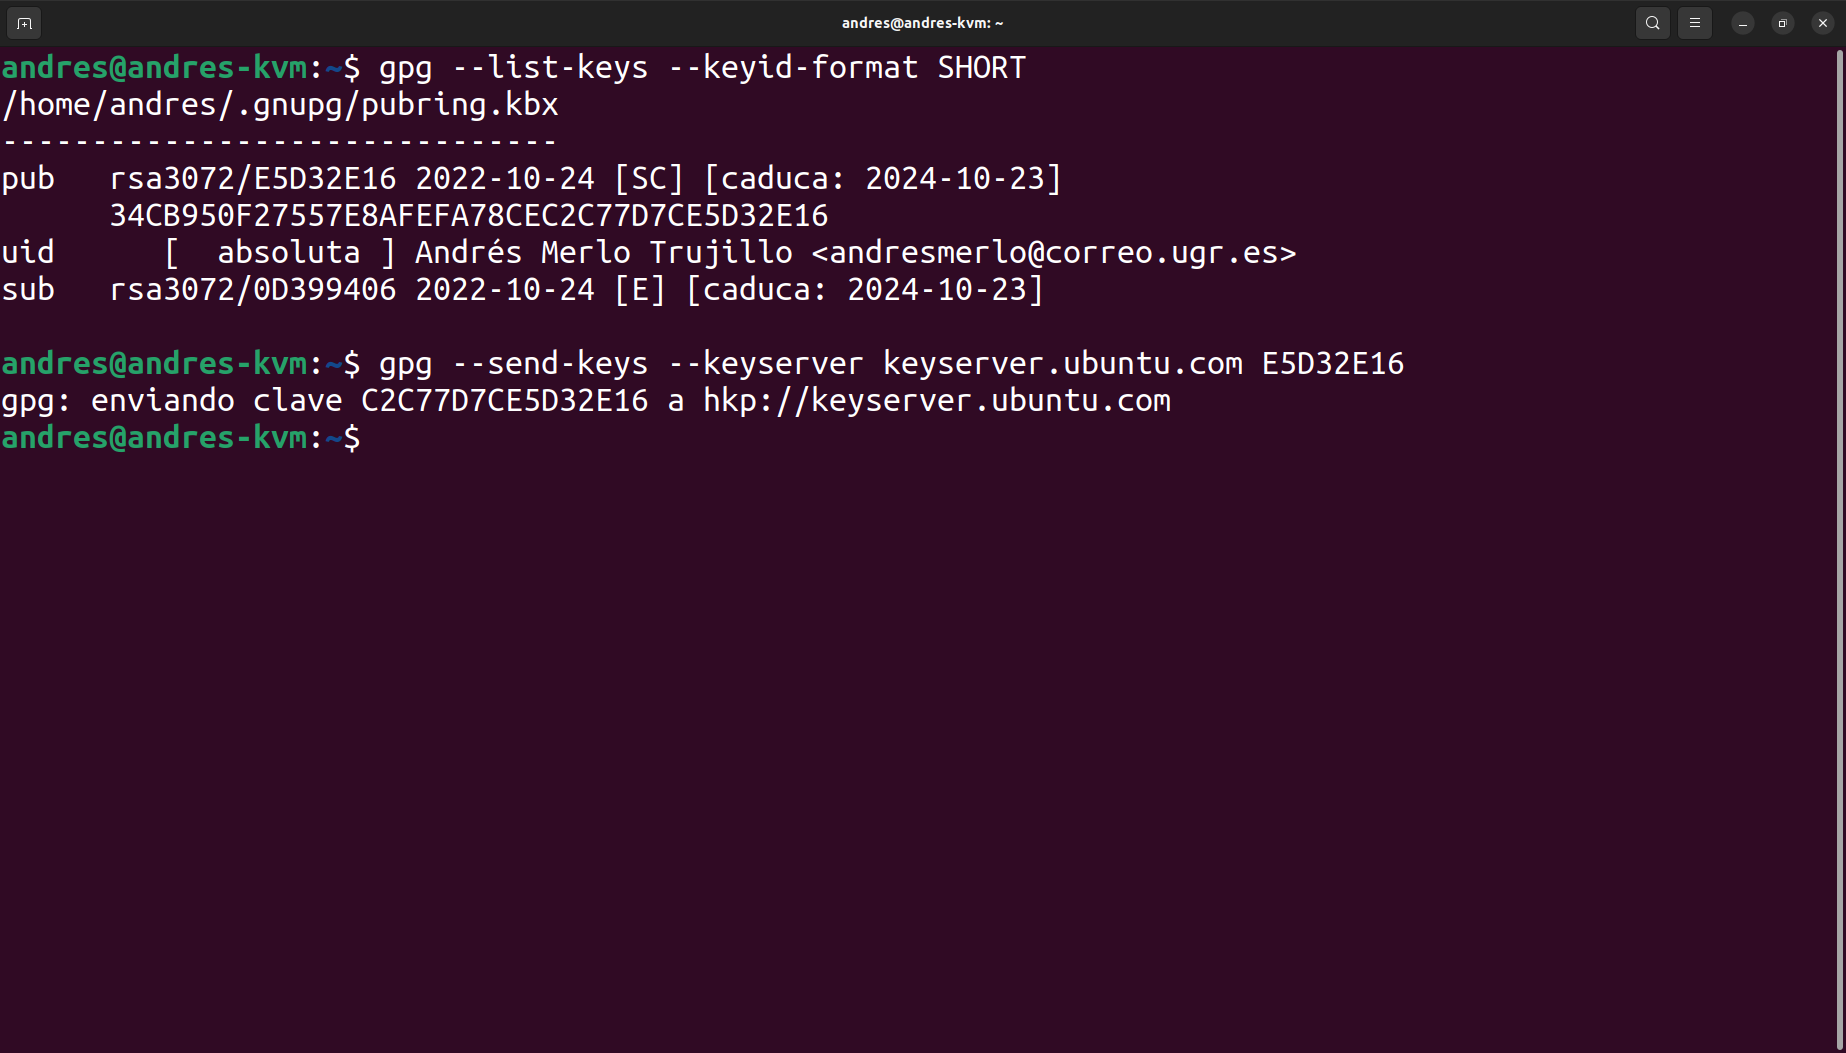
\includegraphics[width=\textwidth]{imagenes/Portatil/Captura desde 2022-10-24 11-58-08.png}
\end{figure}

Y si todo se ha realizado correctamente, al buscar my clave publica en el servidor deberia aparecer:


\begin{figure}[H]
    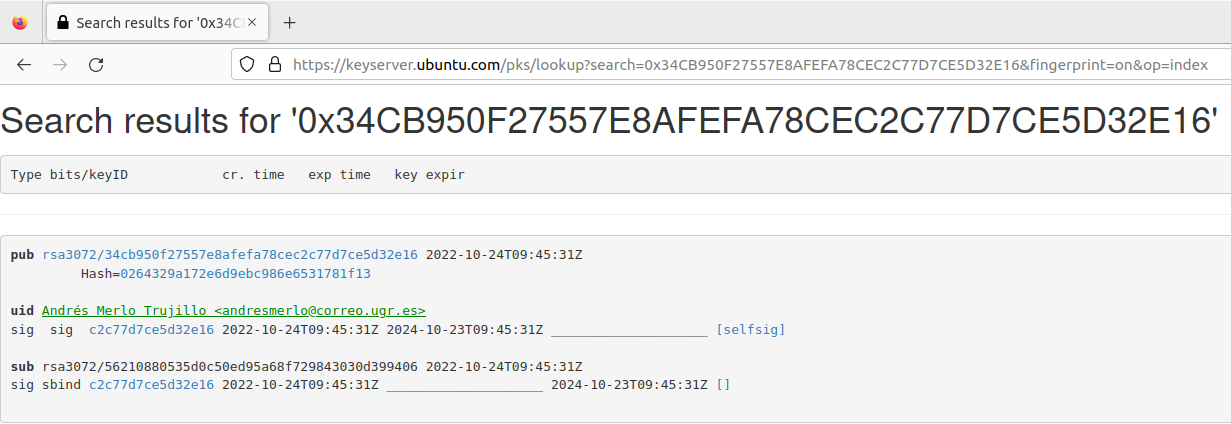
\includegraphics[width=\textwidth]{imagenes/Portatil/Captura desde 2022-10-24 12-01-53.png}
\end{figure}

Y mi compañero tambien ha subido la suya:

\begin{figure}[H]
    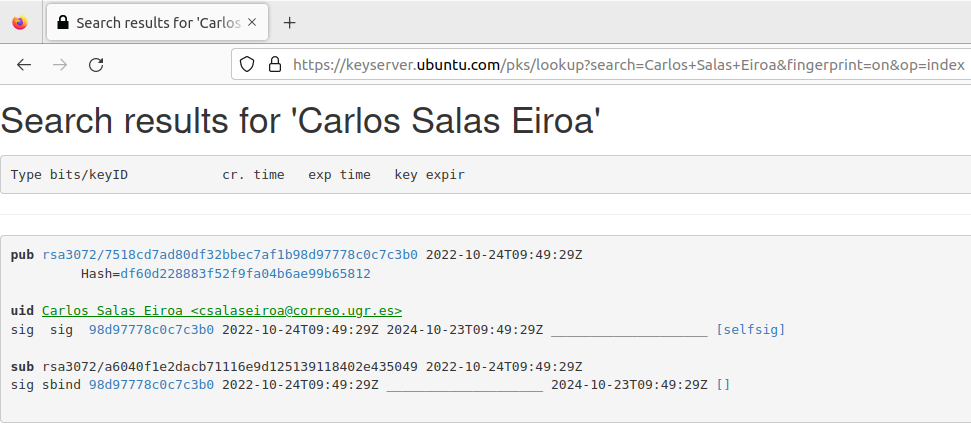
\includegraphics[width=\textwidth]{imagenes/Portatil/Captura desde 2022-10-24 12-05-30.png}
\end{figure}


A continuacion, he creado el siguiente archivo para mi compañero:

\begin{figure}[H]
    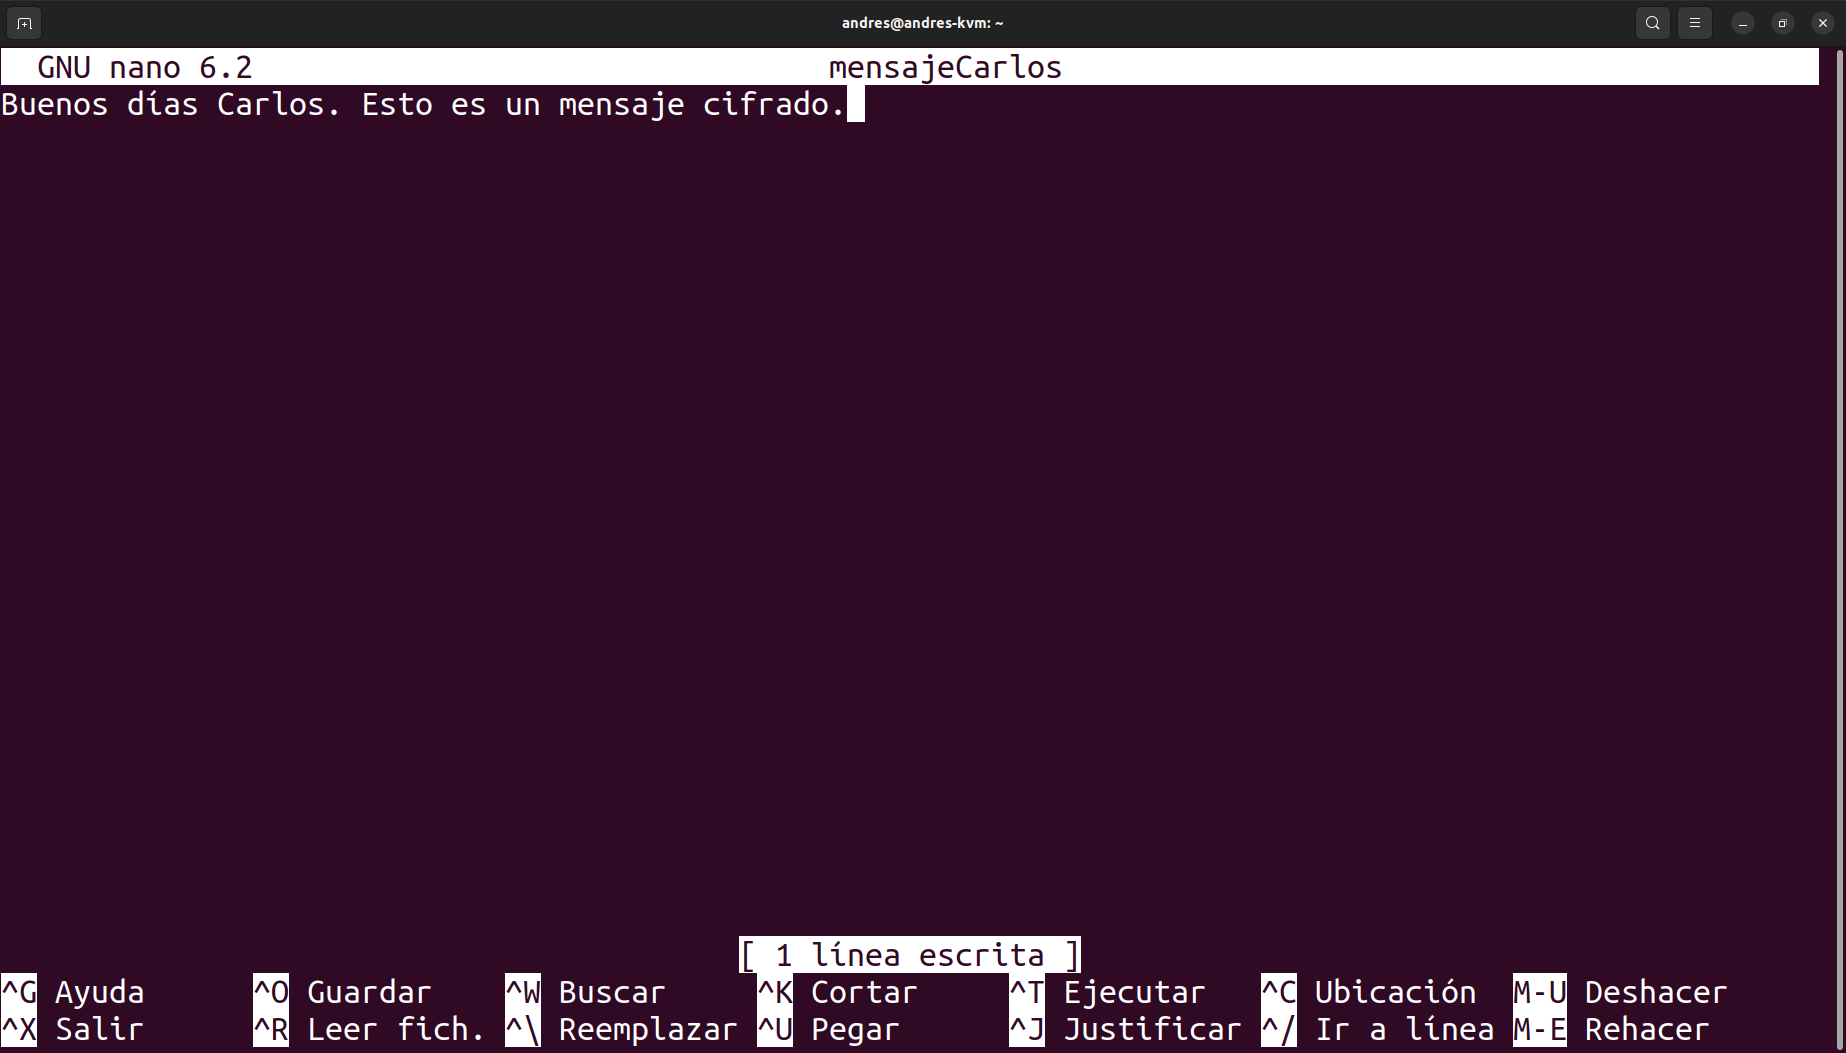
\includegraphics[width=\textwidth]{imagenes/Portatil/Captura desde 2022-10-24 12-02-33.png}
\end{figure}

Y necesito su clave publica del servidor para poder encriptarlo y que solo el pueda leerlo, para ello, con el comando \verb|gpg --keyserver keyserver.ubuntu.com --recv-keys SHORT_ID| obtengo su clave publica:

\begin{figure}[H]
    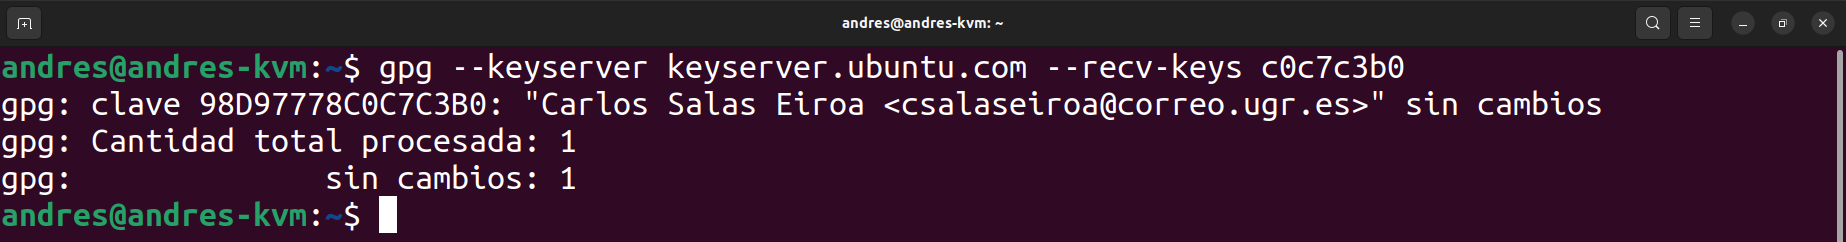
\includegraphics[width=\textwidth]{imagenes/Portatil/Captura desde 2022-10-24 12-11-03.png}
\end{figure}

Y con la orden \verb|gpg --armor --recipient correo --encrypt file| se encripta y se puede mandar el archivo con extension ``.asc'' sin problema por correo electronico.

\begin{figure}[H]
    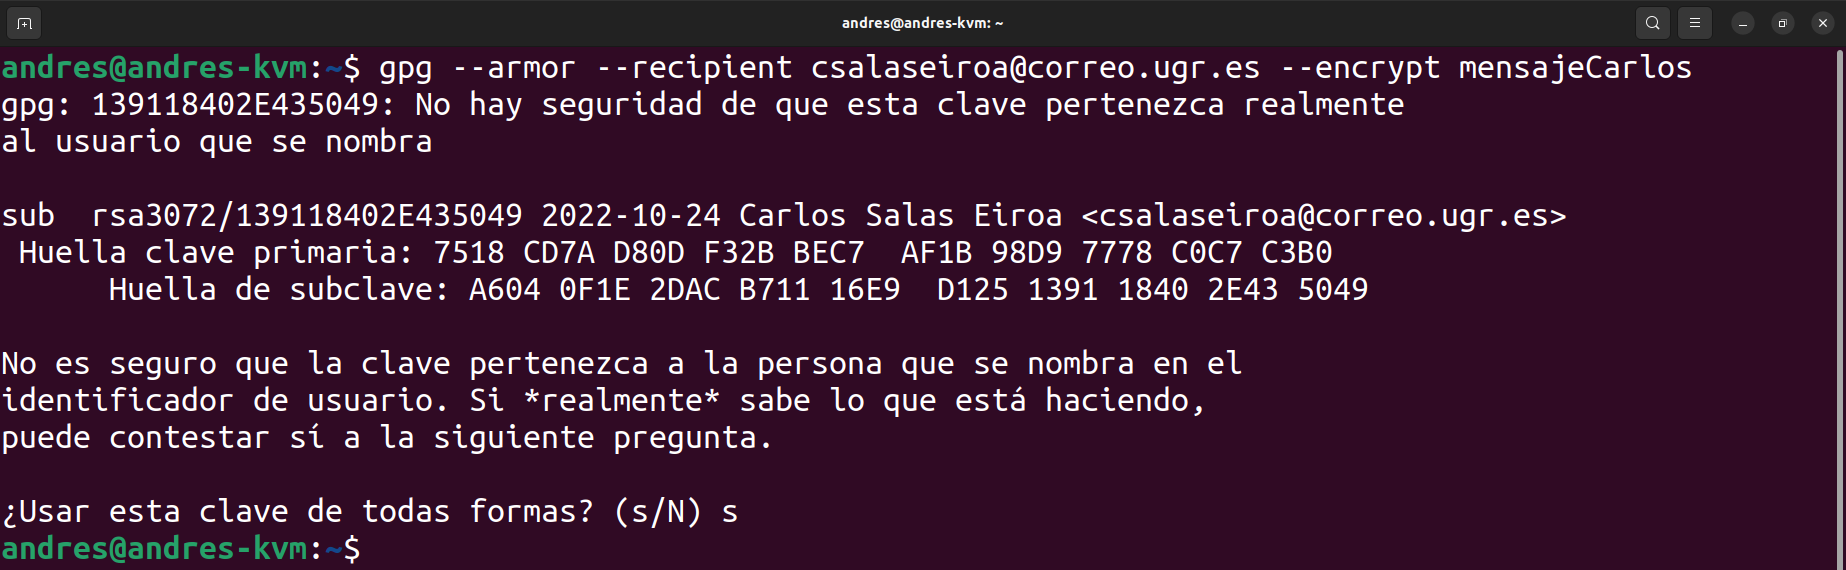
\includegraphics[width=\textwidth]{imagenes/Portatil/Captura desde 2022-10-24 12-11-31.png}
\end{figure}

Ahora, me descargo el archivo que mi compañero me ha enviado por correo electronico:

\begin{figure}[H]
    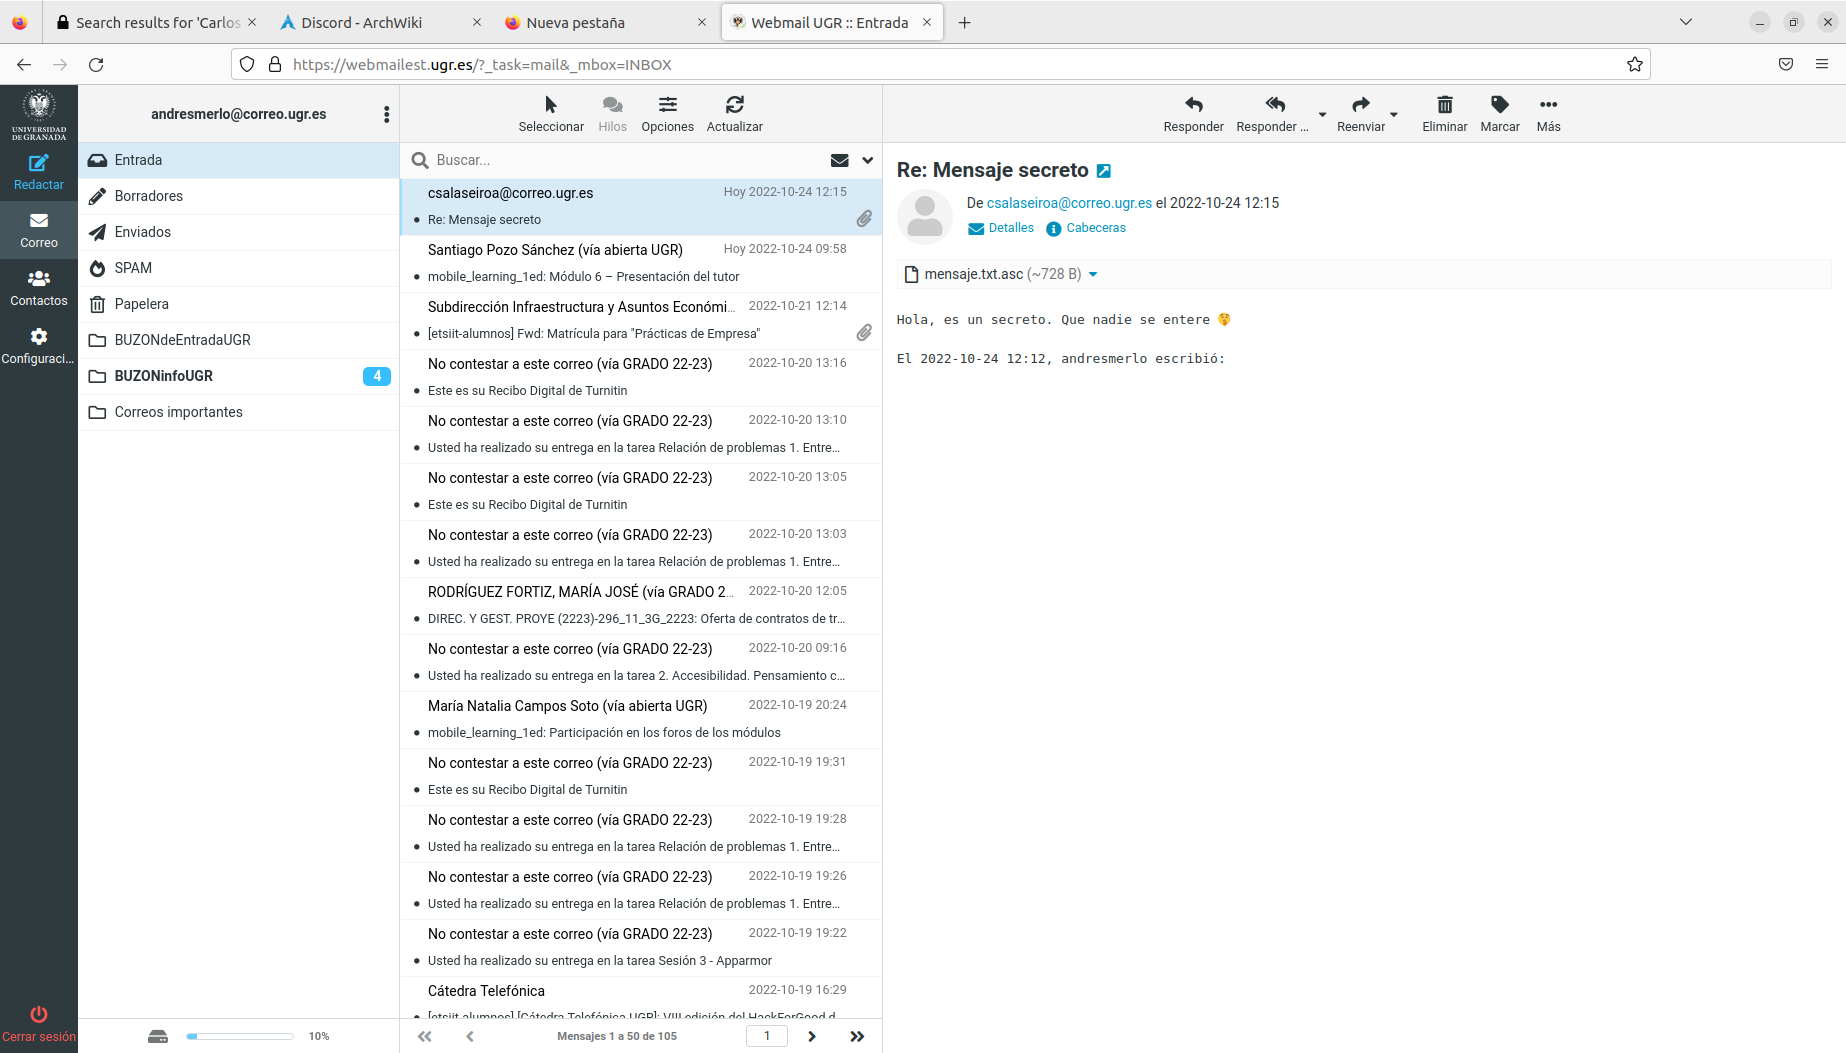
\includegraphics[width=\textwidth]{imagenes/Portatil/Captura desde 2022-10-24 12-16-48.png}
\end{figure}

A continuacion, usando la orden \verb|gpg --decrypt file| se puede abrir el archivo que mi compañero me ha enviado.

\begin{figure}[H]
    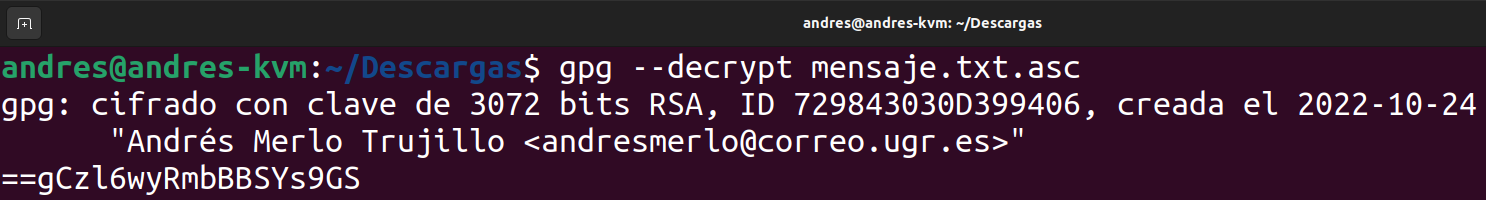
\includegraphics[width=\textwidth]{imagenes/Portatil/Captura desde 2022-10-24 12-18-40.png}
\end{figure}

Como se puede ver, tambien ha ``encriptado'' el mensaje del interior, se puede observar que al principio tiene dos simbolos ``='', señal de que ha usado base64 y le ha dado la vuelta. Para desencriptarlo del todo, es necesario usar la orden \verb|echo "msg" | rev | base64 -d|:

\begin{figure}[H]
    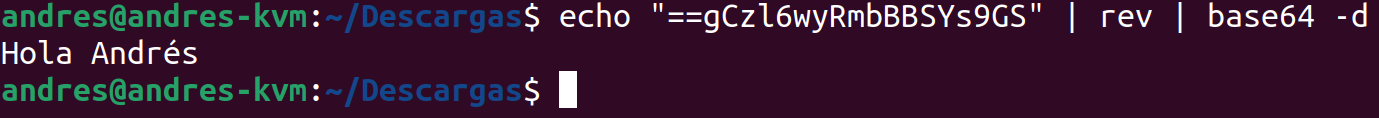
\includegraphics[width=\textwidth]{imagenes/Portatil/base64.png}
\end{figure}

Y finalmente se puede leer el mensaje sin problema alguno.

\addcontentsline{toc}{section}{Ejercicio 2}
\section*{Ejercicio 2}

Voy a cifrar el siguiente archivo:

%Captura desde 2022-10-19 17-33-08
\begin{figure}[H]
    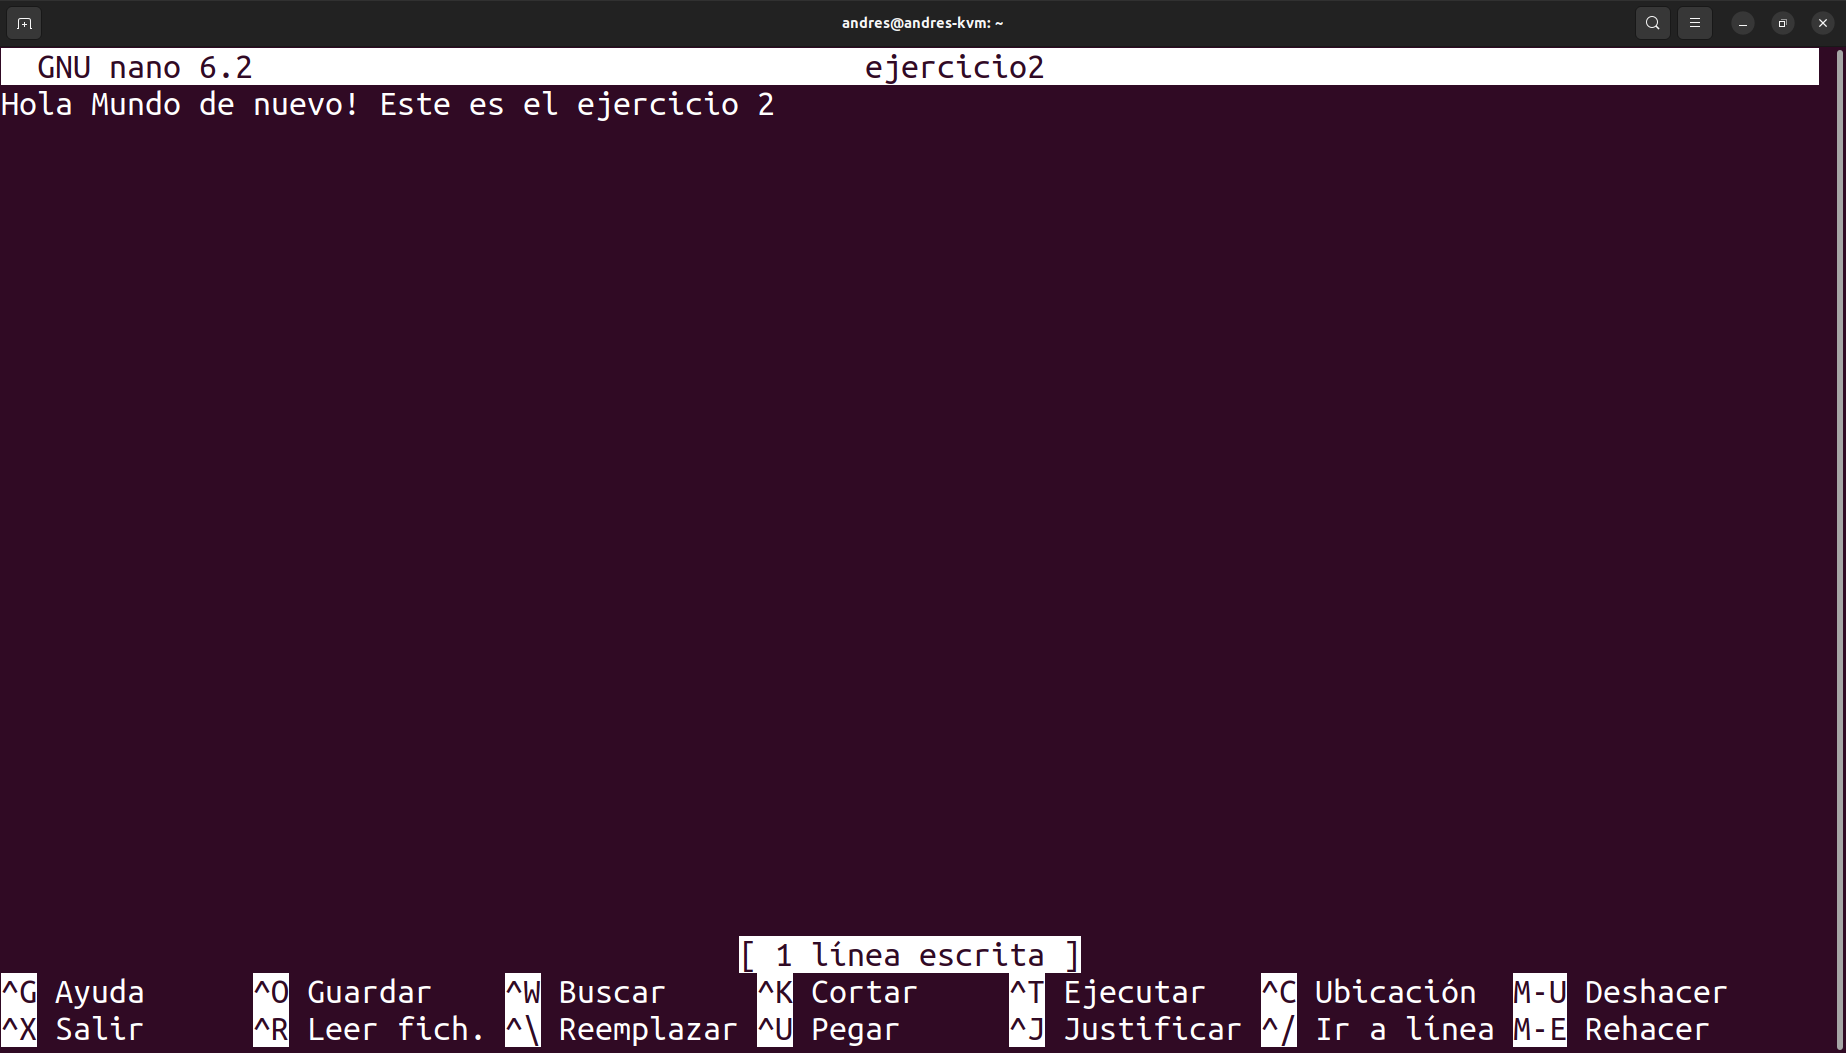
\includegraphics[width=\textwidth]{imagenes/Captura desde 2022-10-19 17-33-08.png}
\end{figure}

El algoritmo de cifrado que voy a usar es ``desx'' y voy a usar 1234 iteraciones y con la contraseña ``qwerty''. Por tanto, para realizar esto, es necesario usar la orden \verb|openssl enc -des3 -iter 1234 -in ejercicio2 -out cifrado|

%Captura desde 2022-10-19 17-44-41
\begin{figure}[H]
    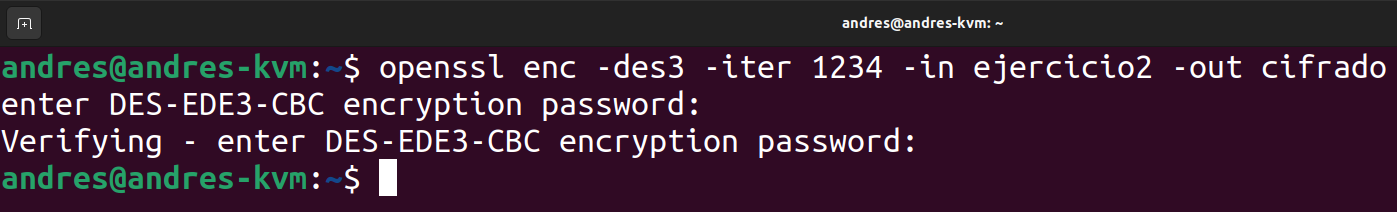
\includegraphics[width=\textwidth]{imagenes/Captura desde 2022-10-19 17-44-41.png}
\end{figure}

COmo se puede observar, pide la contraseña para encriptar, que es ``qwerty'' como he dicho antes. 

Ahora al mostrar el contenido del archivo cifrado, se ve que no es entendible:

%Captura desde 2022-10-19 17-44-49
\begin{figure}[H]
    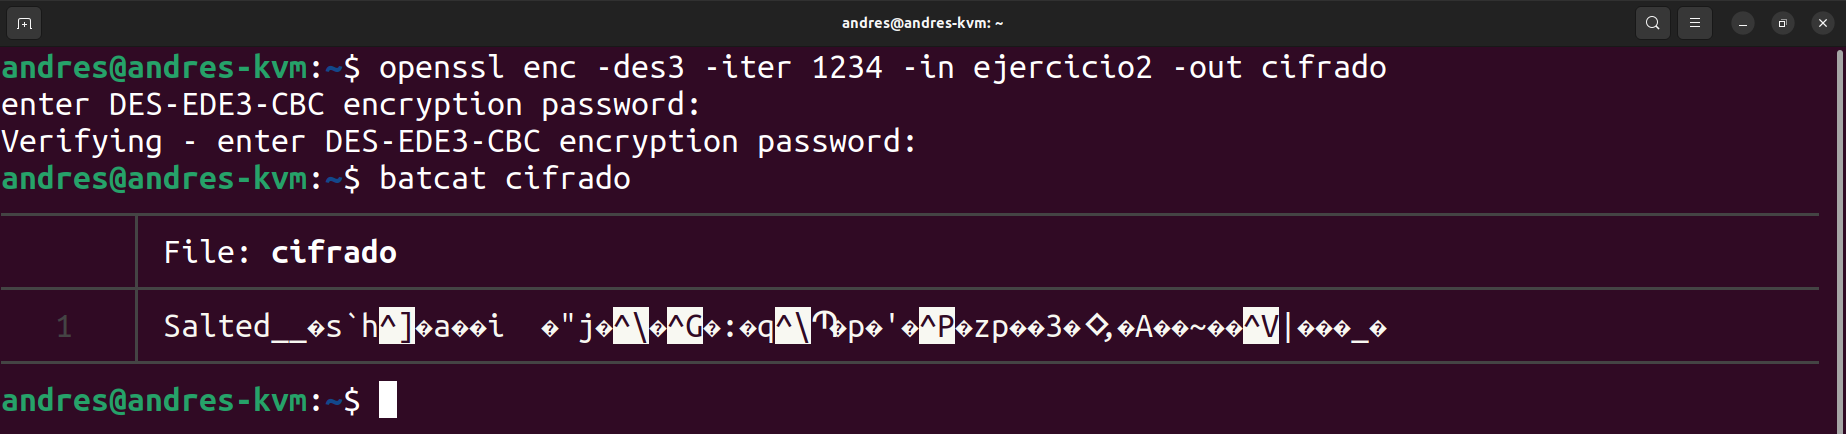
\includegraphics[width=\textwidth]{imagenes/Captura desde 2022-10-19 17-44-49.png}
\end{figure}


Y ahora para descifrarlo, simplemente hace falta saber la contraseña, el algoritmo de cifrado y el numero de iteraciones. Todo esto se debe poner en el siguiente comando: \verb|openssl enc -des3 -iter 1234 -d -in cifrado|

%Captura desde 2022-10-19 17-54-02
\begin{figure}[H]
    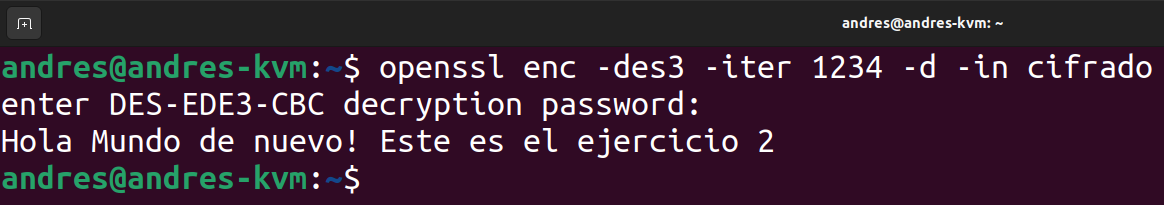
\includegraphics[width=\textwidth]{imagenes/Captura desde 2022-10-19 17-54-02.png}
\end{figure}

\end{document}

%\begin{figure}[H]
%    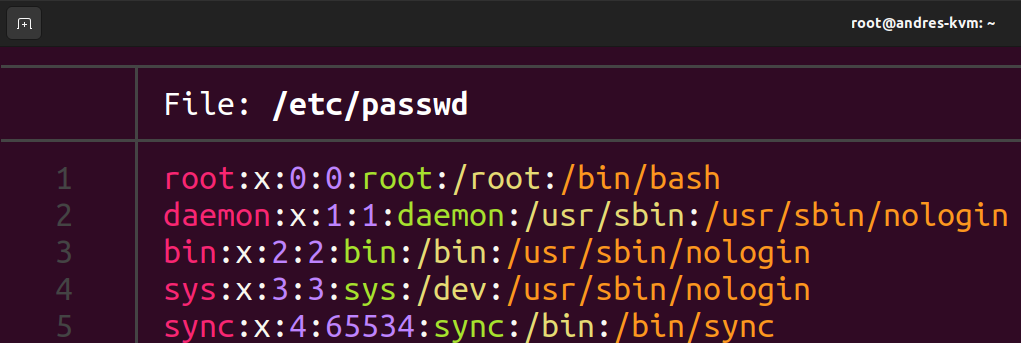
\includegraphics[width=\textwidth]{imagenes/passwdfile.png}
%    \caption{Ejemplo de entradas en el archivo.}
%\end{figure}